% =====================================================================
% SOICT 2026 — 7-minute oral presentation
% Paper: papers/soict2026/manuscript/main.tex
% Compile: ./compile.sh   (XeLaTeX; notes version via NOTES=1 ./compile.sh)
%
% TIMING PLAN (~7:30 total). Three section pages sit between
% the parts; they are not frame-numbered and cost ~5 s each to click past.
%   Title .......................... 0:20
%   I   Problem, contributions ..... 1:25   (2 slides)
%   II  Architecture, modes ........ 1:40   (2 slides)
%   III Results, conclusion ........ 3:55   (5 slides)
% About 7:30 in total with Result 3 (the gate trade-off). If held strictly
% to 7:00, skip Result 2 (the Grafana view) and say its one-line conclusion.
% Slides after the references are BACKUP for Q&A.
% Speaker notes live in \note{} — build them with NOTES=1.
% =====================================================================
\documentclass[aspectratio=169, 11pt]{beamer}
% =====================================================================
% Shared Beamer preamble for all decks in slides/
%   - 16:9, metropolis theme, Okabe-Ito colorblind-safe accents
%   - XeLaTeX + fontspec with a Vietnamese-capable sans fallback chain
%   - Speaker notes: compile with \def\shownotes{} to get the notes PDF
% Input this file right after \documentclass in each deck.
% =====================================================================

\usetheme{metropolis}
\metroset{block=fill, numbering=fraction, progressbar=frametitle, sectionpage=progressbar}

\usepackage{fontspec}
\usepackage{graphicx}
\usepackage{booktabs}
\usepackage{multirow}
\usepackage{amsmath,amssymb}
\usepackage{xcolor}
\usepackage{tikz}
\usetikzlibrary{positioning, arrows.meta, shapes.geometric, fit, backgrounds, calc}
\usepackage{appendixnumberbeamer}

% ---------------------------------------------------------------------
% Fonts. TeX Gyre Heros is the portable first choice (ships with a full
% TeX Live and covers Vietnamese); on a BasicTeX/macOS box it is absent,
% so fall back to system sans fonts that still carry Vietnamese
% diacritics, and only as a last resort to the serif TeX Gyre Termes
% (which is always present) rather than silently hitting nullfont.
% ---------------------------------------------------------------------
\IfFontExistsTF{TeX Gyre Heros}
  {\setsansfont{TeX Gyre Heros}[Ligatures=TeX]}
  {\IfFontExistsTF{Helvetica Neue}
     {\setsansfont{Helvetica Neue}[Ligatures=TeX]}
     {\IfFontExistsTF{Arial}
        {\setsansfont{Arial}[Ligatures=TeX]}
        {\setsansfont{TeX Gyre Termes}[Ligatures=TeX]}}}
\IfFontExistsTF{Menlo}
  {\setmonofont{Menlo}[Scale=0.82]}
  {\IfFontExistsTF{TeX Gyre Cursor}{\setmonofont{TeX Gyre Cursor}[Scale=0.85]}{}}

% ---------------------------------------------------------------------
% Palette. Blue and green follow the Okabe-Ito accents used in the
% manuscript TikZ figures; the emphasis accent is a red rather than
% Okabe-Ito's vermillion, so highlighted numbers read unambiguously as
% "look here" from the back of the room.
% ---------------------------------------------------------------------
\definecolor{accBlue}{HTML}{0072B2}
\definecolor{accGreen}{HTML}{009E73}
\definecolor{accRed}{HTML}{C1121F}
\definecolor{inkDark}{HTML}{23373B}

\setbeamercolor{frametitle}{bg=accBlue, fg=white}
\setbeamercolor{progress bar}{fg=accRed, bg=accRed!25}
\setbeamercolor{progress bar in head/foot}{fg=accRed, bg=accBlue!25}
\setbeamercolor{progress bar in section page}{fg=accRed, bg=accRed!25}
\setbeamercolor{alerted text}{fg=accRed}
\setbeamercolor{example text}{fg=accGreen}
\setbeamercolor{block title}{bg=accBlue!12, fg=inkDark}
\setbeamercolor{block body}{bg=accBlue!5}
\setbeamercolor{block title alerted}{bg=accRed!15, fg=inkDark}
\setbeamercolor{block body alerted}{bg=accRed!6}
\setbeamercolor{block title example}{bg=accGreen!15, fg=inkDark}
\setbeamercolor{block body example}{bg=accGreen!6}

% [standout] frames: metropolis paints them dark teal. Use the same blue as
% the frame titles so the closing slide reads as part of the same deck, and
% size the text up — it is meant to be seen from the back of the room.
\setbeamercolor{palette primary}{bg=accBlue, fg=white}
\setbeamerfont{standout}{size=\huge, series=\bfseries}

% Metropolis draws no bullet glyph by default; a small square reads better
% from the back of a conference room than pure indentation.
\setbeamertemplate{itemize item}{\raisebox{0.12ex}{\tiny$\blacksquare$}}
\setbeamertemplate{itemize subitem}{\raisebox{0.12ex}{\tiny$\square$}}
\setbeamercolor{itemize item}{fg=accBlue}
\setbeamercolor{itemize subitem}{fg=accBlue!70}

% Vietnamese has few hyphenation points, so a long run of words can fail to
% break and stick out past the text block. Allow looser interword glue as a
% last resort instead of an overfull line.
\setlength{\emergencystretch}{2em}

% Tables: booktabs rules look thin on a projector.
\setlength{\heavyrulewidth}{1.1pt}
\setlength{\lightrulewidth}{0.6pt}
\renewcommand{\arraystretch}{1.15}

% ---------------------------------------------------------------------
% Centre the title page and the section pages. Metropolis left-aligns both
% (\raggedright inside its templates); all three decks here want them
% centred, so each calls \centeredtitles right after loading this file.
% It stays a macro rather than an unconditional override so a future deck
% can keep the stock metropolis alignment by simply not calling it.
% ---------------------------------------------------------------------
\makeatletter
\newcommand{\centeredtitles}{%
  % Applied through \AtBeginDocument: metropolis re-applies its own inner
  % templates at \begin{document}, so overrides installed earlier are
  % silently reverted.
  \AtBeginDocument{%
    % Metropolis' title page puts the title graphic in a \vbox to 0pt at the
    % very top of a bottom-aligned \paperheight minipage — the image loads but
    % lands off the top of the page. Rebuild the title page with the graphic
    % after the opening \vfill, where it is actually visible.
    \setbeamertemplate{title graphic}{}%
    \setbeamertemplate{title page}{%
      \begin{minipage}[b][\paperheight]{\textwidth}
        \vfill
        \centering
        \ifx\inserttitlegraphic\@empty\else
          \inserttitlegraphic\par\vspace*{1.1em}%
        \fi
        \ifx\inserttitle\@empty\else\usebeamertemplate*{title}\fi
        \ifx\insertsubtitle\@empty\else\usebeamertemplate*{subtitle}\fi
        \usebeamertemplate*{title separator}
        \ifx\beamer@shortauthor\@empty\else\usebeamertemplate*{author}\fi
        \ifx\insertdate\@empty\else\usebeamertemplate*{date}\fi
        \ifx\insertinstitute\@empty\else\usebeamertemplate*{institute}\fi
        \vfill
        \vspace*{1mm}
      \end{minipage}}%
    \setbeamertemplate{title}{%
      \centering\linespread{1.0}\inserttitle\par\vspace*{0.5em}}%
    \setbeamertemplate{subtitle}{%
      \centering\insertsubtitle\par\vspace*{0.5em}}%
    \setbeamertemplate{author}{%
      \vspace*{2em}\centering\insertauthor\par\vspace*{0.25em}}%
    \setbeamertemplate{date}{%
      \centering\insertdate\par}%
    \setbeamertemplate{institute}{%
      \vspace*{3mm}\centering\insertinstitute\par}%
    % Same as metropolis' "progressbar" section page, but centred. No deck
    % here uses subsections, so that branch of the original is dropped.
    \setbeamertemplate{section page}{%
      \centering
      \begin{minipage}{22em}
        \centering
        \usebeamercolor[fg]{section title}%
        \usebeamerfont{section title}%
        \insertsectionhead\\[-1ex]
        \usebeamertemplate*{progress bar in section page}%
        \par
      \end{minipage}
      \par
      \vspace{\baselineskip}}%
  }%
}
\makeatother

% Shrink a box to the available width, but only when it would otherwise
% overflow. A tabular that is wider than its beamer column is NOT clipped —
% it silently overprints the neighbouring column — so every table that sits
% inside \begin{columns} goes through this.
\newcommand{\fitwidth}[1]{%
  \resizebox{\ifdim\width>\linewidth\linewidth\else\width\fi}{!}{#1}}

% ---------------------------------------------------------------------
% Emphasis macros used throughout the decks.
% ---------------------------------------------------------------------
\newcommand{\key}[1]{\textcolor{accBlue}{\textbf{#1}}}
\newcommand{\good}[1]{\textcolor{accGreen}{\textbf{#1}}}
\newcommand{\bad}[1]{\textcolor{accRed}{\textbf{#1}}}
\newcommand{\num}[1]{\textcolor{accRed}{\textbf{#1}}}

% One-line "so what" strip, pinned at the bottom of a result slide.
% Kept deliberately compact: this box sits directly above metropolis' frame
% number, so any extra height here pushes text into the footer and the page
% number ends up printed on top of the last line.
\newcommand{\takeaway}[1]{%
  \vfill
  \begin{beamercolorbox}[wd=\textwidth, sep=4pt, rounded=true]{block body example}%
    \footnotesize #1%
  \end{beamercolorbox}}

% ---------------------------------------------------------------------
% Speaker notes. Build the plain deck normally; build the notes version
% with:  xelatex "\def\shownotes{}% =====================================================================
% SOICT 2026 — 7-minute oral presentation
% Paper: papers/soict2026/manuscript/main.tex
% Compile: ./compile.sh   (XeLaTeX; notes version via NOTES=1 ./compile.sh)
%
% TIMING PLAN (~7:30 total). Three section pages sit between
% the parts; they are not frame-numbered and cost ~5 s each to click past.
%   Title .......................... 0:20
%   I   Problem, contributions ..... 1:25   (2 slides)
%   II  Architecture, modes ........ 1:40   (2 slides)
%   III Results, conclusion ........ 3:55   (5 slides)
% About 7:30 in total with Result 3 (the gate trade-off). If held strictly
% to 7:00, skip Result 2 (the Grafana view) and say its one-line conclusion.
% Slides after the references are BACKUP for Q&A.
% Speaker notes live in \note{} — build them with NOTES=1.
% =====================================================================
\documentclass[aspectratio=169, 11pt]{beamer}
% =====================================================================
% Shared Beamer preamble for all decks in slides/
%   - 16:9, metropolis theme, Okabe-Ito colorblind-safe accents
%   - XeLaTeX + fontspec with a Vietnamese-capable sans fallback chain
%   - Speaker notes: compile with \def\shownotes{} to get the notes PDF
% Input this file right after \documentclass in each deck.
% =====================================================================

\usetheme{metropolis}
\metroset{block=fill, numbering=fraction, progressbar=frametitle, sectionpage=progressbar}

\usepackage{fontspec}
\usepackage{graphicx}
\usepackage{booktabs}
\usepackage{multirow}
\usepackage{amsmath,amssymb}
\usepackage{xcolor}
\usepackage{tikz}
\usetikzlibrary{positioning, arrows.meta, shapes.geometric, fit, backgrounds, calc}
\usepackage{appendixnumberbeamer}

% ---------------------------------------------------------------------
% Fonts. TeX Gyre Heros is the portable first choice (ships with a full
% TeX Live and covers Vietnamese); on a BasicTeX/macOS box it is absent,
% so fall back to system sans fonts that still carry Vietnamese
% diacritics, and only as a last resort to the serif TeX Gyre Termes
% (which is always present) rather than silently hitting nullfont.
% ---------------------------------------------------------------------
\IfFontExistsTF{TeX Gyre Heros}
  {\setsansfont{TeX Gyre Heros}[Ligatures=TeX]}
  {\IfFontExistsTF{Helvetica Neue}
     {\setsansfont{Helvetica Neue}[Ligatures=TeX]}
     {\IfFontExistsTF{Arial}
        {\setsansfont{Arial}[Ligatures=TeX]}
        {\setsansfont{TeX Gyre Termes}[Ligatures=TeX]}}}
\IfFontExistsTF{Menlo}
  {\setmonofont{Menlo}[Scale=0.82]}
  {\IfFontExistsTF{TeX Gyre Cursor}{\setmonofont{TeX Gyre Cursor}[Scale=0.85]}{}}

% ---------------------------------------------------------------------
% Palette. Blue and green follow the Okabe-Ito accents used in the
% manuscript TikZ figures; the emphasis accent is a red rather than
% Okabe-Ito's vermillion, so highlighted numbers read unambiguously as
% "look here" from the back of the room.
% ---------------------------------------------------------------------
\definecolor{accBlue}{HTML}{0072B2}
\definecolor{accGreen}{HTML}{009E73}
\definecolor{accRed}{HTML}{C1121F}
\definecolor{inkDark}{HTML}{23373B}

\setbeamercolor{frametitle}{bg=accBlue, fg=white}
\setbeamercolor{progress bar}{fg=accRed, bg=accRed!25}
\setbeamercolor{progress bar in head/foot}{fg=accRed, bg=accBlue!25}
\setbeamercolor{progress bar in section page}{fg=accRed, bg=accRed!25}
\setbeamercolor{alerted text}{fg=accRed}
\setbeamercolor{example text}{fg=accGreen}
\setbeamercolor{block title}{bg=accBlue!12, fg=inkDark}
\setbeamercolor{block body}{bg=accBlue!5}
\setbeamercolor{block title alerted}{bg=accRed!15, fg=inkDark}
\setbeamercolor{block body alerted}{bg=accRed!6}
\setbeamercolor{block title example}{bg=accGreen!15, fg=inkDark}
\setbeamercolor{block body example}{bg=accGreen!6}

% [standout] frames: metropolis paints them dark teal. Use the same blue as
% the frame titles so the closing slide reads as part of the same deck, and
% size the text up — it is meant to be seen from the back of the room.
\setbeamercolor{palette primary}{bg=accBlue, fg=white}
\setbeamerfont{standout}{size=\huge, series=\bfseries}

% Metropolis draws no bullet glyph by default; a small square reads better
% from the back of a conference room than pure indentation.
\setbeamertemplate{itemize item}{\raisebox{0.12ex}{\tiny$\blacksquare$}}
\setbeamertemplate{itemize subitem}{\raisebox{0.12ex}{\tiny$\square$}}
\setbeamercolor{itemize item}{fg=accBlue}
\setbeamercolor{itemize subitem}{fg=accBlue!70}

% Vietnamese has few hyphenation points, so a long run of words can fail to
% break and stick out past the text block. Allow looser interword glue as a
% last resort instead of an overfull line.
\setlength{\emergencystretch}{2em}

% Tables: booktabs rules look thin on a projector.
\setlength{\heavyrulewidth}{1.1pt}
\setlength{\lightrulewidth}{0.6pt}
\renewcommand{\arraystretch}{1.15}

% ---------------------------------------------------------------------
% Centre the title page and the section pages. Metropolis left-aligns both
% (\raggedright inside its templates); all three decks here want them
% centred, so each calls \centeredtitles right after loading this file.
% It stays a macro rather than an unconditional override so a future deck
% can keep the stock metropolis alignment by simply not calling it.
% ---------------------------------------------------------------------
\makeatletter
\newcommand{\centeredtitles}{%
  % Applied through \AtBeginDocument: metropolis re-applies its own inner
  % templates at \begin{document}, so overrides installed earlier are
  % silently reverted.
  \AtBeginDocument{%
    % Metropolis' title page puts the title graphic in a \vbox to 0pt at the
    % very top of a bottom-aligned \paperheight minipage — the image loads but
    % lands off the top of the page. Rebuild the title page with the graphic
    % after the opening \vfill, where it is actually visible.
    \setbeamertemplate{title graphic}{}%
    \setbeamertemplate{title page}{%
      \begin{minipage}[b][\paperheight]{\textwidth}
        \vfill
        \centering
        \ifx\inserttitlegraphic\@empty\else
          \inserttitlegraphic\par\vspace*{1.1em}%
        \fi
        \ifx\inserttitle\@empty\else\usebeamertemplate*{title}\fi
        \ifx\insertsubtitle\@empty\else\usebeamertemplate*{subtitle}\fi
        \usebeamertemplate*{title separator}
        \ifx\beamer@shortauthor\@empty\else\usebeamertemplate*{author}\fi
        \ifx\insertdate\@empty\else\usebeamertemplate*{date}\fi
        \ifx\insertinstitute\@empty\else\usebeamertemplate*{institute}\fi
        \vfill
        \vspace*{1mm}
      \end{minipage}}%
    \setbeamertemplate{title}{%
      \centering\linespread{1.0}\inserttitle\par\vspace*{0.5em}}%
    \setbeamertemplate{subtitle}{%
      \centering\insertsubtitle\par\vspace*{0.5em}}%
    \setbeamertemplate{author}{%
      \vspace*{2em}\centering\insertauthor\par\vspace*{0.25em}}%
    \setbeamertemplate{date}{%
      \centering\insertdate\par}%
    \setbeamertemplate{institute}{%
      \vspace*{3mm}\centering\insertinstitute\par}%
    % Same as metropolis' "progressbar" section page, but centred. No deck
    % here uses subsections, so that branch of the original is dropped.
    \setbeamertemplate{section page}{%
      \centering
      \begin{minipage}{22em}
        \centering
        \usebeamercolor[fg]{section title}%
        \usebeamerfont{section title}%
        \insertsectionhead\\[-1ex]
        \usebeamertemplate*{progress bar in section page}%
        \par
      \end{minipage}
      \par
      \vspace{\baselineskip}}%
  }%
}
\makeatother

% Shrink a box to the available width, but only when it would otherwise
% overflow. A tabular that is wider than its beamer column is NOT clipped —
% it silently overprints the neighbouring column — so every table that sits
% inside \begin{columns} goes through this.
\newcommand{\fitwidth}[1]{%
  \resizebox{\ifdim\width>\linewidth\linewidth\else\width\fi}{!}{#1}}

% ---------------------------------------------------------------------
% Emphasis macros used throughout the decks.
% ---------------------------------------------------------------------
\newcommand{\key}[1]{\textcolor{accBlue}{\textbf{#1}}}
\newcommand{\good}[1]{\textcolor{accGreen}{\textbf{#1}}}
\newcommand{\bad}[1]{\textcolor{accRed}{\textbf{#1}}}
\newcommand{\num}[1]{\textcolor{accRed}{\textbf{#1}}}

% One-line "so what" strip, pinned at the bottom of a result slide.
% Kept deliberately compact: this box sits directly above metropolis' frame
% number, so any extra height here pushes text into the footer and the page
% number ends up printed on top of the last line.
\newcommand{\takeaway}[1]{%
  \vfill
  \begin{beamercolorbox}[wd=\textwidth, sep=4pt, rounded=true]{block body example}%
    \footnotesize #1%
  \end{beamercolorbox}}

% ---------------------------------------------------------------------
% Speaker notes. Build the plain deck normally; build the notes version
% with:  xelatex "\def\shownotes{}\input{main.tex}"
% ---------------------------------------------------------------------
\ifdefined\shownotes
  \usepackage{pgfpages}
  \setbeameroption{show notes on second screen=right}
\fi

\centeredtitles

\graphicspath{%
  {../../papers/soict2026/results/remeasure_20260930/}%
  {../../papers/soict2026/results/benchmarks/}%
  {../../papers/soict2026/figures/}%
  {../../results/ml_08_anomaly_gate/}%
  {../../results/ml_07_cross_method_comparison/}%
}

\title{A Distributed Real-Time Intrusion Detection System on a Jetson Orin Nano Super Edge Cluster using Kafka and PySpark}
\author{\textbf{Thai Nguyen Vu}\inst{1} \and Dung Van Bui\inst{2} \and Nhut Tri Do\inst{2} \and Van Du Nguyen\inst{3}}
\institute{\scriptsize
           \inst{1}Campus in Ho Chi Minh City, University of Transport and Communications, Ho Chi Minh City, Vietnam \\
           \inst{2}University of Information Technology, VNU-HCM, Ho Chi Minh City, Vietnam \\
           \inst{3}Faculty of Information Technology, Nong Lam University, Ho Chi Minh City, Vietnam}
\date{SOICT 2026}

\begin{document}

% ---------------------------------------------------------------- 0:20
\maketitle
\note{Good morning. I will show what a second edge board actually buys you
when you split an ML intrusion detector across two Jetson Orin Nano Super
devices. Seven minutes, four results.}

% ---------------------------------------------------------------- 0:50
% =====================================================================
\section{I.\ PROBLEM AND CONTRIBUTIONS}
% =====================================================================

\begin{frame}{Edge intrusion detection: three open gaps}
  \begin{columns}[T]
    \begin{column}{0.55\textwidth}
      Detectors now \emph{fit} on single-board hardware --- but a monolithic
      one classifies \key{every} flow and saturates an 8\,GB ARM board.
      \vspace{0.6em}

      \textbf{What the literature does not tell us}
      \begin{enumerate}
        \item Everything is measured on a \bad{single device}.
        \item Throughput, latency and \bad{energy} are never reported together.
        \item Offline scores come from \bad{leaky protocols}.
      \end{enumerate}
    \end{column}
    \begin{column}{0.42\textwidth}
      \begin{alertblock}{Our question}
        How should inference be \emph{placed} across a constrained two-node
        edge cluster?
      \end{alertblock}
      \begin{exampleblock}{Our answer}
        Split it: a cheap \key{autoencoder gate} on board \#1, the heavy
        \key{PySpark classifier} on board \#2, joined by a Kafka topic.
      \end{exampleblock}
    \end{column}
  \end{columns}
  \note{Three gaps: single-device evaluation, energy never reported next to
  latency, and offline numbers taken from leaky pipelines. Which model to
  deploy is the other half of the question. We attack all three with one
  system.}
\end{frame}

% ---------------------------------------------------------------- 0:35
\begin{frame}{Contributions}
  \begin{enumerate}
    \item A \key{two-stage distributed IDS}: anomaly gate $+$ Spark classifier,
          physically separated across two boards.
    \item \key{Three deployment modes} for a two-node Jetson cluster ---
          pipeline split, horizontal Kafka scaling, Spark standalone cluster.
    \item An \key{end-to-end evaluation}: throughput, latency percentiles,
          per-node CPU/RAM \emph{and} energy per verdict.
    \item \key{Leakage-aware provenance} --- the deployed model is exactly the
          one our companion study selected under a leakage-free protocol.
  \end{enumerate}
  \note{Four contributions. The fourth matters: the model we deploy is not a
  fresh model, it is the one that survived a strict offline audit.}
\end{frame}

% ---------------------------------------------------------------- 1:00
% =====================================================================
\section{II.\ SYSTEM AND EVALUATION SETUP}
% =====================================================================

\begin{frame}{Split-deployment architecture}
  \centering
  \resizebox{0.70\textwidth}{!}{%
  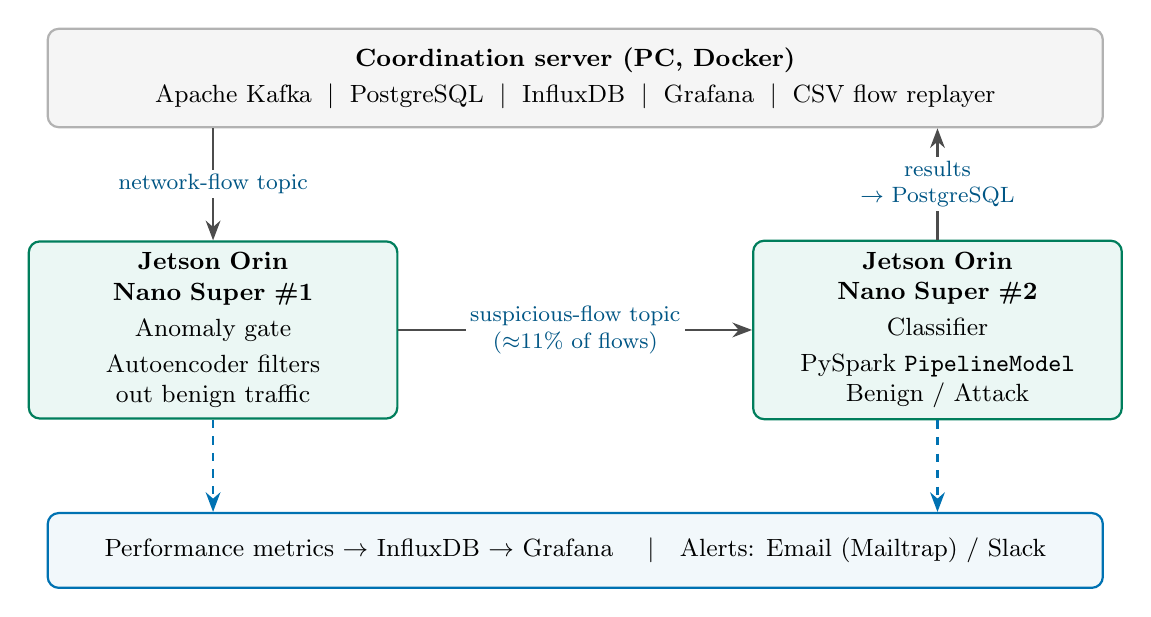
\begin{tikzpicture}[
      font=\small, >=Stealth, every node/.style={align=center},
      pc/.style ={draw=gray!60, thick, rounded corners, fill=gray!8, minimum width=13.4cm, minimum height=1.25cm, inner sep=3pt},
      jet/.style={draw=accGreen!80!black, thick, rounded corners, fill=accGreen!8, text width=4.4cm, minimum height=1.9cm, inner sep=4pt},
      mtr/.style={draw=accBlue, thick, rounded corners, fill=accBlue!5, minimum width=13.4cm, minimum height=0.95cm, inner sep=3pt},
      lbl/.style={font=\footnotesize, fill=white, inner sep=1.5pt, align=center, text=accBlue!75!black},
      arr/.style={-{Stealth[length=2.5mm]}, thick, draw=gray!60!black},
      dsh/.style={-{Stealth[length=2.5mm]}, thick, draw=accBlue, dashed},
  ]
    \node[pc]  (pc)  at (0, 0.0)   {\textbf{Coordination server (PC, Docker)}\\[2pt]
        Apache Kafka \;$|$\; PostgreSQL \;$|$\; InfluxDB \;$|$\; Grafana \;$|$\; CSV flow replayer};
    \node[jet] (j1)  at (-4.6,-3.2) {\textbf{Jetson Orin Nano Super \#1}\\[2pt] \key{Anomaly gate}\\[2pt]
        Autoencoder filters out benign traffic};
    \node[jet] (j2)  at ( 4.6,-3.2) {\textbf{Jetson Orin Nano Super \#2}\\[2pt] \key{Classifier}\\[2pt]
        PySpark \texttt{PipelineModel}\\ Benign / Attack};
    \node[mtr] (out) at (0,-6.0)   {Performance metrics $\rightarrow$ InfluxDB $\rightarrow$ Grafana \quad$|$\quad
        Alerts: Email (Mailtrap) / Slack};
    \draw[arr] (pc.south -| j1) -- node[lbl]{network-flow topic} (j1.north);
    \draw[arr] (j1.east) -- node[lbl]{suspicious-flow topic\\ ($\approx$11\% of flows)} (j2.west);
    \draw[arr] (j2.north) -- node[lbl]{results\\ $\rightarrow$ PostgreSQL} (pc.south -| j2);
    \draw[dsh] (j1.south) -- (out.north -| j1);
    \draw[dsh] (j2.south) -- (out.north -| j2);
  \end{tikzpicture}}
  \\[0.15em]
  \footnotesize The gate scores all 77 features; its threshold is fixed
  \emph{offline} on benign validation data, never on the test set. Batches of
  20, or after 1\,s.
  \\[0.2em]
  {\tiny\textcolor{gray!55!black}{CICIDS2017: Sharafaldin et al., ICISSP 2018
  $\cdot$ Kafka: Kreps et al., NetDB 2011 $\cdot$ Spark: Zaharia et al.,
  HotCloud 2010.}}
  \note{Host runs the infrastructure. Board one gates, board two classifies.
  Only suspicious flows cross the Kafka topic between them. Everything is
  instrumented into Grafana.}
\end{frame}

% ---------------------------------------------------------------- 0:40
\begin{frame}{Deployment modes and what we measure}
  \begin{columns}[T]
    \begin{column}{0.58\textwidth}
      \begin{description}\small
        \item[Single node] full pipeline on one board, gate off or on.
        \item[A: Pipeline split] gate on \#1, classifier on \#2 (our design).
        \item[B: Horizontal] both boards run the full role (gate off).
        \item[C: Spark cluster] host as master, both boards as workers.
      \end{description}
      \vspace{0.3em}
      \footnotesize \key{Every flow is followed from send to verdict}, queueing
      included. \key{Sustained capacity}: the highest rate at which every flow
      gets its verdict within 10\,s of the load.
    \end{column}
    \begin{column}{0.40\textwidth}
      \begin{block}{Setup}
        \footnotesize
        2$\times$ Jetson Orin Nano Super\\ (6-core A78AE, 8\,GB, $\approx$67\,TOPS)\\[0.3em]
        PySpark 3.4.1, Kafka 3.5, Wi-Fi LAN\\[0.3em]
        10{,}000 test-split flows, 15\% attacks\\[0.3em]
        Rate sweep 1--40 flows/s, 2 runs each\\[0.3em]
        Energy via \texttt{tegrastats}
      \end{block}
    \end{column}
  \end{columns}
  \note{Latency is measured from the moment a flow is sent to the moment its
  verdict is written, so time spent waiting in a queue counts. A fresh Kafka
  consumer group per run, so no run inherits another's backlog.}
\end{frame}

% ---------------------------------------------------------------- 1:20
% =====================================================================
\section{III.\ RESULTS AND CONCLUSION}
% =====================================================================

\begin{frame}{Result 1: splitting the pipeline sustains 9$\times$ the load}
  \begin{columns}[T]
    \begin{column}{0.58\textwidth}
      \centering\small
      \fitwidth{%
      \begin{tabular}{lccc}
        \toprule
        Mode & Flows/s & e2e p95 (s) & J / verdict \\
        \midrule
        Single node         & 2.5            & 11.3          & 3.04 \\
        Single node + gate  & 1.9            & 7.8           & 3.04 \\
        B: Horizontal       & 3.3            & 8.2           & 3.20 \\
        C: Spark cluster    & 8.7            & 5.2           & 1.15 \\
        \textbf{A: Split}   & \num{22.4}     & \num{7.1}     & \num{0.60} \\
        \bottomrule
      \end{tabular}
      }
      \\[0.3em]
      \raggedright\scriptsize
      \textbf{Flows/s}: sustained, every flow done within 10\,s.
      \textbf{e2e p95}: send to verdict, queueing included.
    \end{column}
    \begin{column}{0.39\textwidth}
      \begin{itemize}\small
        \setlength{\itemsep}{0.4em}
        \item \good{Split: 9$\times$ a single node, 5$\times$ less energy per
              verdict.}
        \item \bad{The same gate on the same board gains nothing}: the second
              board is what pays.
        \item Tail latency is seconds: one PySpark batch takes seconds.
      \end{itemize}
    \end{column}
  \end{columns}
  \takeaway{\textbf{Pipeline split is the recommended default}: highest
  sustained load at the lowest energy per verdict.}
  \note{Single node and horizontal run with the gate off, as in the submitted
  version. Energy is measured at each mode's sustained rate: 2.0, 2.0, 3.9,
  9.5 and 18.4 flows per second. Gate skip is about 89 percent in every gated
  mode. Median latency in split mode is about one second.}
\end{frame}

% ---------------------------------------------------------------- 0:35
\begin{frame}{Result 2: the load asymmetry is visible live}
  \begin{columns}[c]
    \begin{column}{0.63\textwidth}
      \centering
      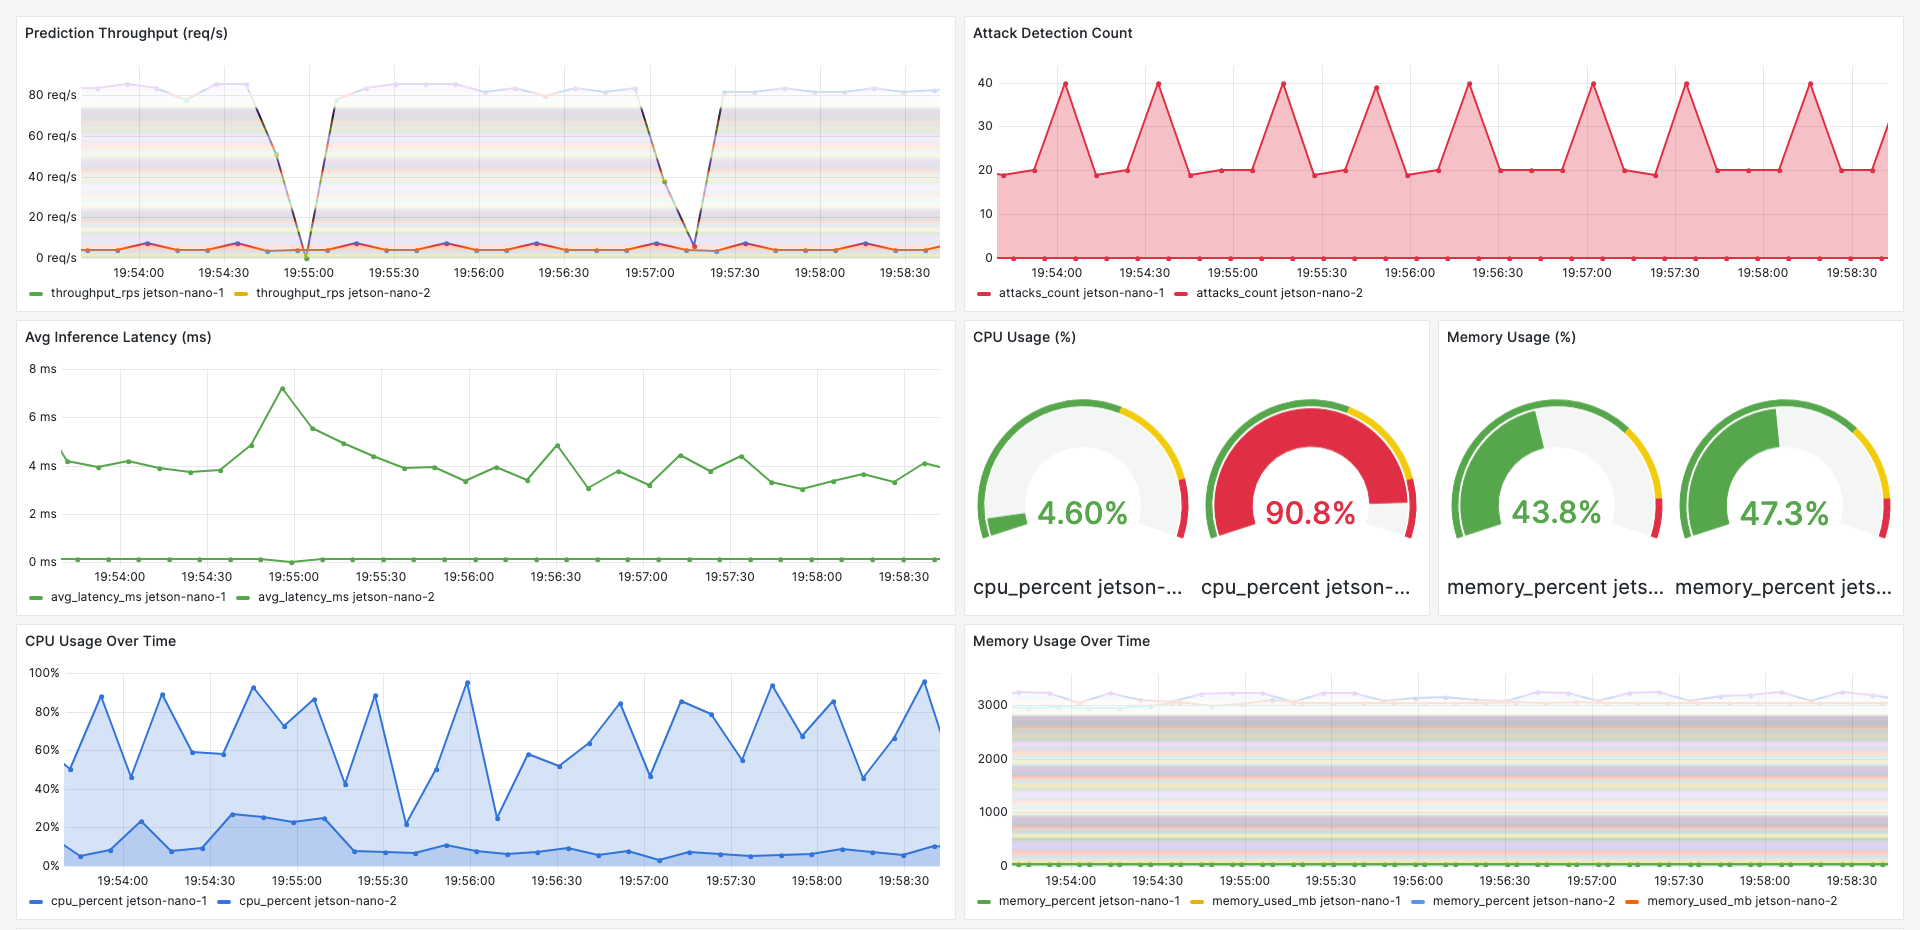
\includegraphics[width=\textwidth]{grafana_peak_load.png}
    \end{column}
    \begin{column}{0.35\textwidth}
      At peak load, split mode\\{\scriptsize (earlier run, previous model)}:
      \begin{itemize}
        \item gate node: \good{4.6\% CPU}
        \item classifier node: \bad{90.8\% CPU}
      \end{itemize}
      \vspace{0.5em}
      The classifier dominates the compute budget --- which is exactly why
      moving it off the ingest path pays.
    \end{column}
  \end{columns}
  \note{Live Grafana at peak load. Under five versus ninety-one percent. The
  asymmetry is the whole argument for the split. Add: the gate is a tunable
  filter, not a fixed point --- backup slide has the operating curve.}
\end{frame}

% ---------------------------------------------------------------- 0:35
\begin{frame}{Result 3: what the gate lets through}
  \begin{columns}[T]
    \begin{column}{0.52\textwidth}
      \centering\small
      \fitwidth{%
      \begin{tabular}{lccc}
        \toprule
        Gate threshold & Attacks & False & Flows \\
        (benign quantile) & forwarded & alarms & skipped \\
        \midrule
        0.99              & 72.4\% & 0.99\% & 88.3\% \\
        \textbf{0.995 (deployed)} & \num{68.1\%} & \num{0.49\%} & 89.4\% \\
        0.999             & 39.8\% & 0.09\% & 94.0\% \\
        \bottomrule
      \end{tabular}
      }
      \\[0.3em]
      \raggedright\scriptsize Offline, CICIDS2017 test split; gate on all 77
      features. Streamed live: 69.6\% of 1{,}261 attack flows caught.
    \end{column}
    \begin{column}{0.45\textwidth}
      \begin{itemize}\small
        \setlength{\itemsep}{0.4em}
        \item A flow the gate skips is final: \bad{about 30\% of attack flows}
              never reach the classifier.
        \item On the classifier's 30 features the gate would forward only
              44.8\%.
        \item The operator picks the point that fits the budget.
      \end{itemize}
    \end{column}
  \end{columns}
  \takeaway{The capacity gain is paid for in recall: the gate is a
  \key{tunable trade-off}, not a free filter.}
  \note{Numbers from results/ml\_08\_anomaly\_gate/gate\_operating\_points.csv;
  the deployed threshold is quantile 0.995. Without the gate, every attack flow
  in the replay was caught, so the loss is the gate's.}
\end{frame}

% ---------------------------------------------------------------- 0:45
\begin{frame}{Result 4: the price of one unified stack}
  We serve with Spark for \emph{consistency with distributed training}.
  What does that cost? The \emph{deployed forest}, exported, same board:
  \vspace{0.5em}
  \centering
  \small
  \fitwidth{%
  \begin{tabular}{lccc}
    \toprule
    Engine & Flows/s & Batch p95 (ms) & mJ per flow \\
    \midrule
    PySpark (deployed) & 1.4      & 7515  & 1506 \\
    NumPy              & 54.8     & 194   & 11.3 \\
    \textbf{ONNX Runtime} & \num{10{,}092} & \num{1.2} & \num{0.087} \\
    \bottomrule
  \end{tabular}
  }
  \\[0.2em]{\scriptsize Identical predictions on every flow. mJ per flow: energy
  above the board's idle power.}
  \takeaway{ONNX Runtime serves the same forest \num{$\approx$7{,}200$\times$}
  faster. Target for the next iteration: \key{train on Spark, serve with
  ONNX/TensorRT}.}
  \note{The JVM costs us more than three orders of magnitude, and that sets
  the roadmap. Batch size 10.}
\end{frame}

% ---------------------------------------------------------------- 0:40
\begin{frame}{Conclusion}
  \begin{columns}[T]
    \begin{column}{0.53\textwidth}
      \textbf{What we showed}
      \begin{itemize}
        \item A reproducible distributed edge IDS: Kafka $+$ PySpark on a
              Jetson Orin Nano Super cluster.
        \item Gate and classifier on separate boards:
              \good{2.5 $\rightarrow$ 22.4 flows/s} sustained, e2e p95
              $\approx$7\,s.
        \item Energy per verdict: \good{3.0\,J $\rightarrow$ 0.60\,J}.
        \item ONNX serves the same forest $\approx$7{,}200$\times$ faster.
      \end{itemize}
    \end{column}
    \begin{column}{0.44\textwidth}
      \textbf{Limitations}
      \begin{itemize}\footnotesize
        \item Two-node lab cluster over Wi-Fi; replayed traffic.
        \item Gate skips $\approx$30\% of attack flows.
        \item GPU unused (CPU-only pipeline); evasion untested.
      \end{itemize}
      \textbf{Next}
      \begin{itemize}\footnotesize
        \item ONNX/TensorRT serving; live traffic; retraining under drift.
      \end{itemize}
    \end{column}
  \end{columns}
  \vfill
  \centering
  \key{Thank you --- questions?}
  \note{Recap: nine times the load, five times less energy per verdict, and
  the price, about thirty percent of attacks skipped by the gate.}
\end{frame}

% ---------------------------------------------------------------- 7:00
\begin{frame}{Key references}
  \begin{itemize}\footnotesize
    \setlength{\itemsep}{0em}
    \item[{[1]}] Sharafaldin, I., Lashkari, A.\,H. \& Ghorbani, A.\,A.
          \emph{Toward generating a new intrusion detection dataset and
          intrusion traffic characterization}. ICISSP 2018.
          \hfill{\key{CICIDS2017}}
    \item[{[2]}] Shi, W. et al. \emph{Edge computing: Vision and challenges}.
          IEEE Internet of Things Journal 3(5), 2016.
          \hfill{\key{edge setting}}
    \item[{[3]}] Chandola, V., Banerjee, A. \& Kumar, V. \emph{Anomaly detection:
          A survey}. ACM Computing Surveys 41(3), 2009.
          \hfill{\key{anomaly gate}}
    \item[{[4]}] Lundberg, S.\,M. \& Lee, S.-I. \emph{A unified approach to
          interpreting model predictions}. NeurIPS 2017.
          \hfill{\key{SHAP Top-30}}
    \item[{[5]}] Zaharia, M. et al. \emph{Spark: Cluster computing with working
          sets}. HotCloud 2010.
          \hfill{\key{Spark}}
    \item[{[6]}] Kreps, J., Narkhede, N. \& Rao, J. \emph{Kafka: a Distributed
          Messaging System for Log Processing}. NetDB 2011.
          \hfill{\key{Kafka}}
    \item[{[7]}] Mohan Kiran Kumar, K. et al. \emph{Distributed Intrusion Detection
          System using Kafka and Spark Streaming}. ICVADV 2025.
          \hfill{\key{closest system}}
    \item[{[8]}] Arp, D. et al. \emph{Dos and Don'ts of Machine Learning in Computer
          Security}. USENIX Security 2022.
          \hfill{\key{leakage-aware protocol}}
  \end{itemize}
  \note{Not presented --- shown while taking questions, so sources are on
  screen if the audience asks. Full list is in the paper.}
\end{frame}

% =====================================================================
\appendix

\begin{frame}[standout]
  Backup slides
\end{frame}

\begin{frame}{Backup: sustained capacity and energy per mode}
  \centering
  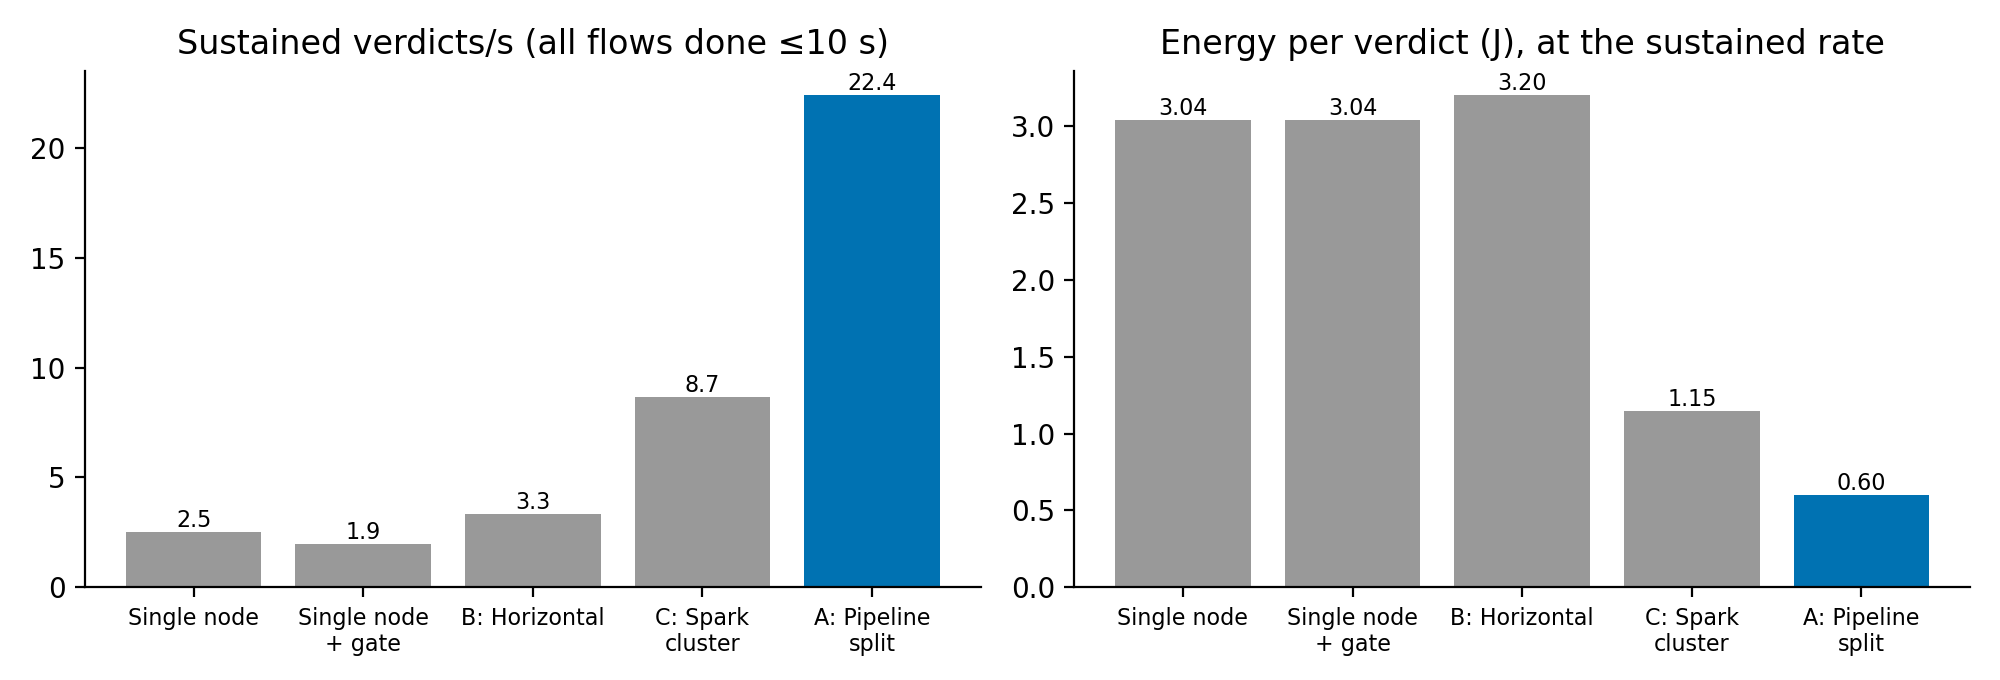
\includegraphics[height=0.70\textheight, width=\textwidth, keepaspectratio]{edge_capacity.png}
  \\[0.2em]
  \footnotesize Sustained verdicts/s with every flow done within 10\,s (left);
  energy per verdict at that rate (right).
\end{frame}

\begin{frame}{Backup: the gate is an operating curve, not a point}
  \centering
  \IfFileExists{../../results/ml_08_anomaly_gate/gate_operating_points.png}
    {\includegraphics[height=0.68\textheight, width=\textwidth, keepaspectratio]{gate_operating_points.png}}
    {\fbox{\parbox{0.7\textwidth}{\centering\vspace{1.5cm}
      \texttt{gate\_operating\_points.png}\vspace{1.5cm}}}}
  \\[0.2em]
  \footnotesize Attack recall (left) and false-positive rate (right) vs.\
  gate-skip ratio. Raising the skip ratio offloads more Spark work and costs
  recall; the operator chooses the point.
\end{frame}

\begin{frame}{Backup: which model, and why}
  \centering\small
  \fitwidth{%
  \begin{tabular}{lcccp{3.3cm}}
    \toprule
    Configuration & F1 & Features & Size (MB) & Edge rationale \\
    \midrule
    Baseline $+$ XGBoost      & 0.9971 & 77 & 2.32 & Reference accuracy \\
    \textbf{SHAP Top-30} $+$ XGBoost & 0.9970 & 30 & 0.003$^{\dagger}$ & Explainable; deployed feature set \\
    RF Top-30 $+$ XGBoost     & 0.9922 & 30 & 2.52 & Embedded ranking \\
    PCA $k$=40 $+$ XGBoost    & 0.9939 & 40 & 3.82 & Unsupervised reduction \\
    \bottomrule
  \end{tabular}
  }
  \\[0.4em]
  \raggedright\footnotesize
  We deploy \key{SHAP Top-30 with Random Forest} (exported model: test F1
  0.9959, 30 features): a native Spark ML estimator, so the
  \texttt{PipelineModel} loads on ARM64 without the native libraries Spark's
  XGBoost integration needs. The SHAP ranking is computed after
  \texttt{destination\_port} is removed.
  \\ $^{\dagger}$Distributed saving under-reports size; true size $\approx$2.5\,MB.
\end{frame}

\begin{frame}{Backup: full monitoring dashboard}
  \centering
  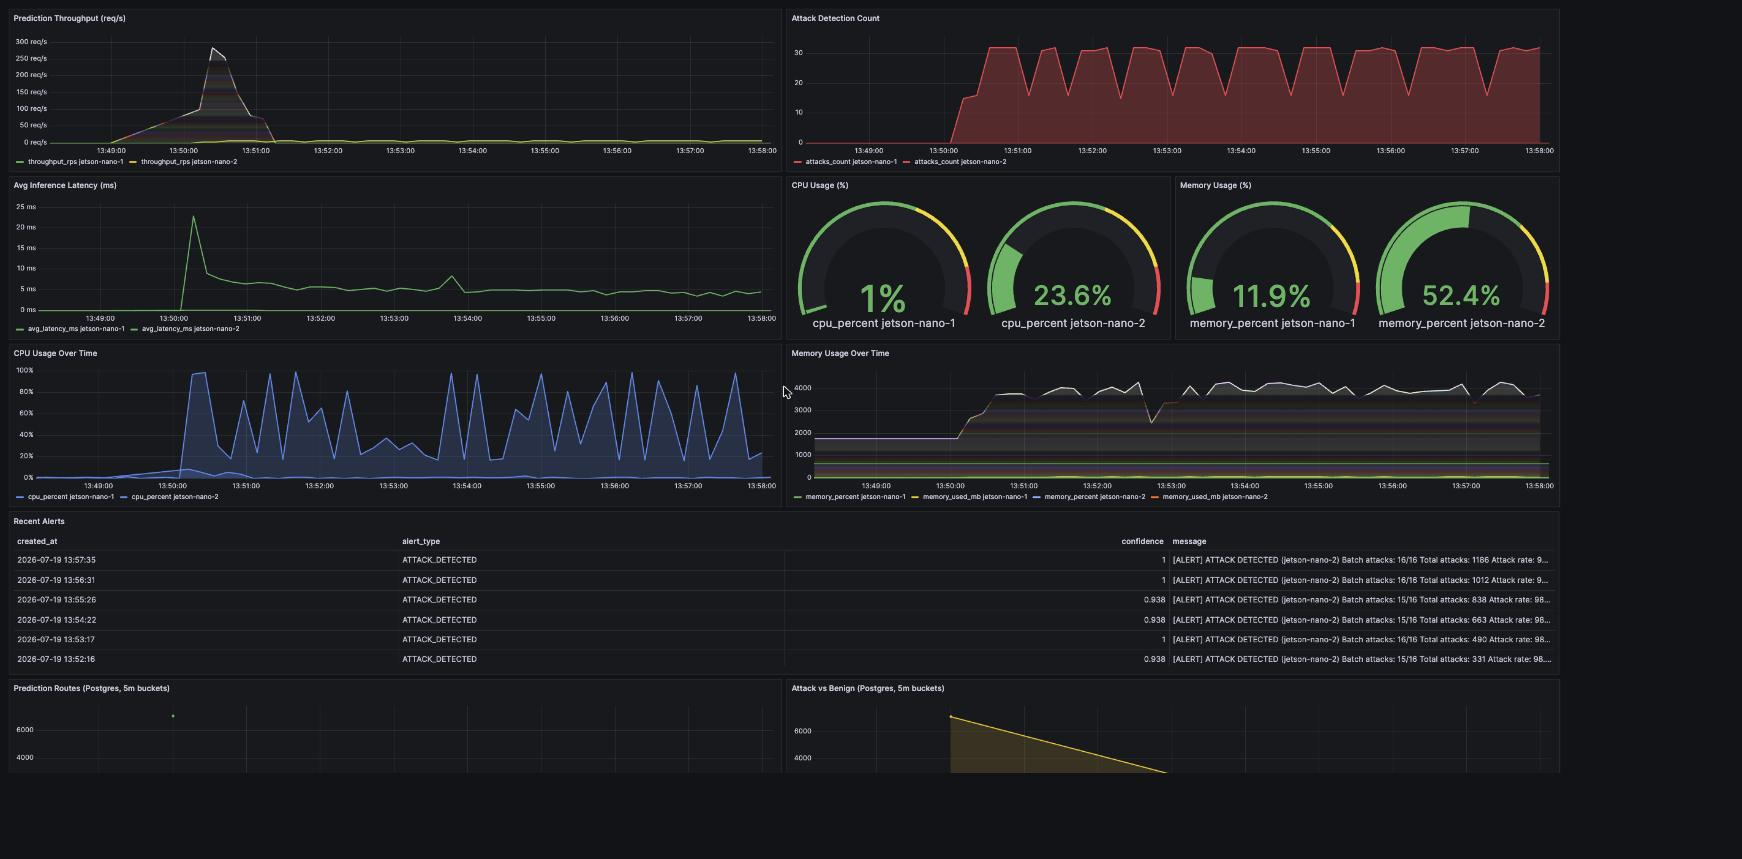
\includegraphics[height=0.70\textheight, width=\textwidth, keepaspectratio]{grafana_dashboard.png}
  \\[0.2em]
  \footnotesize Per-node throughput, detected attacks, inference latency,
  CPU/RAM for both boards, PostgreSQL-backed alerts.
\end{frame}

\begin{frame}{Backup: measurement protocol}
  \begin{itemize}\small
    \item Host-side orchestration starts pipeline roles on the Jetsons over
          SSH, drives the load, collects every verdict.
    \item Each verdict stores the flow's send time and replay row: latency is
          send to verdict, \emph{queueing included}; skip ratio and attack
          recall come from the flows themselves.
    \item Rate sweep per mode; a rate is sustained when every flow sent in the
          45\,s window gets its verdict within 10\,s after it. 2 runs per rate.
    \item Fresh Kafka consumer group per run, so no run inherits a backlog.
    \item Tiers batch 20 flows or flush after 1\,s.
    \item Energy: \texttt{tegrastats}, 30\,s idle baseline then load at the
          sustained rate; two-node modes sum both boards.
  \end{itemize}
\end{frame}

\end{document}
"
% ---------------------------------------------------------------------
\ifdefined\shownotes
  \usepackage{pgfpages}
  \setbeameroption{show notes on second screen=right}
\fi

\centeredtitles

\graphicspath{%
  {../../papers/soict2026/results/remeasure_20260930/}%
  {../../papers/soict2026/results/benchmarks/}%
  {../../papers/soict2026/figures/}%
  {../../results/ml_08_anomaly_gate/}%
  {../../results/ml_07_cross_method_comparison/}%
}

\title{A Distributed Real-Time Intrusion Detection System on a Jetson Orin Nano Super Edge Cluster using Kafka and PySpark}
\author{\textbf{Thai Nguyen Vu}\inst{1} \and Dung Van Bui\inst{2} \and Nhut Tri Do\inst{2} \and Van Du Nguyen\inst{3}}
\institute{\scriptsize
           \inst{1}Campus in Ho Chi Minh City, University of Transport and Communications, Ho Chi Minh City, Vietnam \\
           \inst{2}University of Information Technology, VNU-HCM, Ho Chi Minh City, Vietnam \\
           \inst{3}Faculty of Information Technology, Nong Lam University, Ho Chi Minh City, Vietnam}
\date{SOICT 2026}

\begin{document}

% ---------------------------------------------------------------- 0:20
\maketitle
\note{Good morning. I will show what a second edge board actually buys you
when you split an ML intrusion detector across two Jetson Orin Nano Super
devices. Seven minutes, four results.}

% ---------------------------------------------------------------- 0:50
% =====================================================================
\section{I.\ PROBLEM AND CONTRIBUTIONS}
% =====================================================================

\begin{frame}{Edge intrusion detection: three open gaps}
  \begin{columns}[T]
    \begin{column}{0.55\textwidth}
      Detectors now \emph{fit} on single-board hardware --- but a monolithic
      one classifies \key{every} flow and saturates an 8\,GB ARM board.
      \vspace{0.6em}

      \textbf{What the literature does not tell us}
      \begin{enumerate}
        \item Everything is measured on a \bad{single device}.
        \item Throughput, latency and \bad{energy} are never reported together.
        \item Offline scores come from \bad{leaky protocols}.
      \end{enumerate}
    \end{column}
    \begin{column}{0.42\textwidth}
      \begin{alertblock}{Our question}
        How should inference be \emph{placed} across a constrained two-node
        edge cluster?
      \end{alertblock}
      \begin{exampleblock}{Our answer}
        Split it: a cheap \key{autoencoder gate} on board \#1, the heavy
        \key{PySpark classifier} on board \#2, joined by a Kafka topic.
      \end{exampleblock}
    \end{column}
  \end{columns}
  \note{Three gaps: single-device evaluation, energy never reported next to
  latency, and offline numbers taken from leaky pipelines. Which model to
  deploy is the other half of the question. We attack all three with one
  system.}
\end{frame}

% ---------------------------------------------------------------- 0:35
\begin{frame}{Contributions}
  \begin{enumerate}
    \item A \key{two-stage distributed IDS}: anomaly gate $+$ Spark classifier,
          physically separated across two boards.
    \item \key{Three deployment modes} for a two-node Jetson cluster ---
          pipeline split, horizontal Kafka scaling, Spark standalone cluster.
    \item An \key{end-to-end evaluation}: throughput, latency percentiles,
          per-node CPU/RAM \emph{and} energy per verdict.
    \item \key{Leakage-aware provenance} --- the deployed model is exactly the
          one our companion study selected under a leakage-free protocol.
  \end{enumerate}
  \note{Four contributions. The fourth matters: the model we deploy is not a
  fresh model, it is the one that survived a strict offline audit.}
\end{frame}

% ---------------------------------------------------------------- 1:00
% =====================================================================
\section{II.\ SYSTEM AND EVALUATION SETUP}
% =====================================================================

\begin{frame}{Split-deployment architecture}
  \centering
  \resizebox{0.70\textwidth}{!}{%
  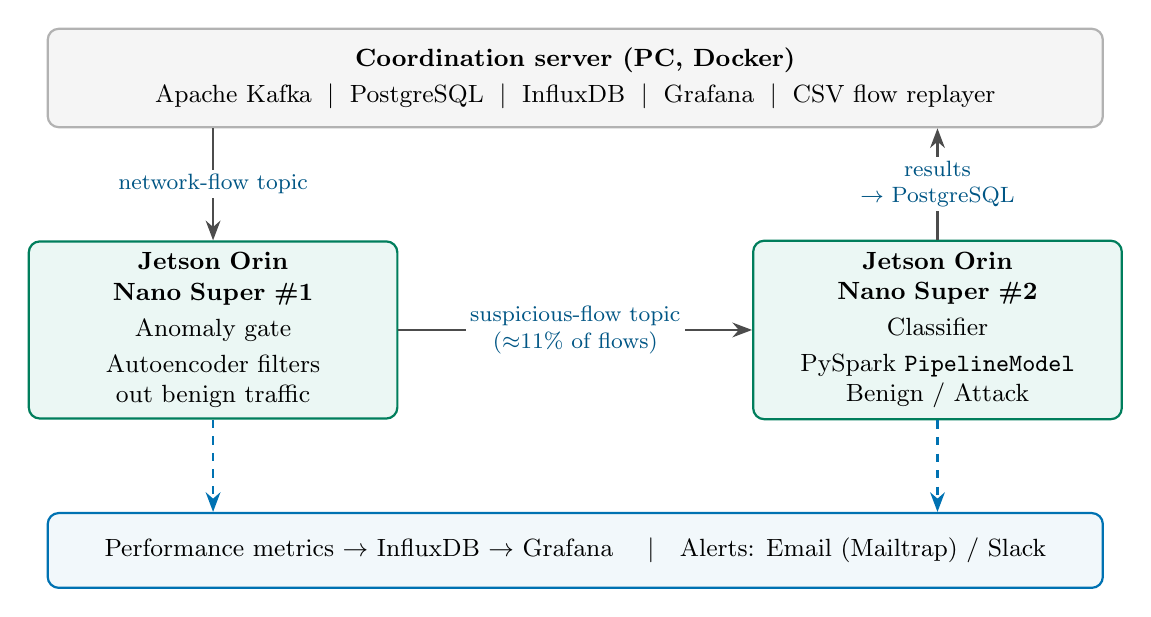
\begin{tikzpicture}[
      font=\small, >=Stealth, every node/.style={align=center},
      pc/.style ={draw=gray!60, thick, rounded corners, fill=gray!8, minimum width=13.4cm, minimum height=1.25cm, inner sep=3pt},
      jet/.style={draw=accGreen!80!black, thick, rounded corners, fill=accGreen!8, text width=4.4cm, minimum height=1.9cm, inner sep=4pt},
      mtr/.style={draw=accBlue, thick, rounded corners, fill=accBlue!5, minimum width=13.4cm, minimum height=0.95cm, inner sep=3pt},
      lbl/.style={font=\footnotesize, fill=white, inner sep=1.5pt, align=center, text=accBlue!75!black},
      arr/.style={-{Stealth[length=2.5mm]}, thick, draw=gray!60!black},
      dsh/.style={-{Stealth[length=2.5mm]}, thick, draw=accBlue, dashed},
  ]
    \node[pc]  (pc)  at (0, 0.0)   {\textbf{Coordination server (PC, Docker)}\\[2pt]
        Apache Kafka \;$|$\; PostgreSQL \;$|$\; InfluxDB \;$|$\; Grafana \;$|$\; CSV flow replayer};
    \node[jet] (j1)  at (-4.6,-3.2) {\textbf{Jetson Orin Nano Super \#1}\\[2pt] \key{Anomaly gate}\\[2pt]
        Autoencoder filters out benign traffic};
    \node[jet] (j2)  at ( 4.6,-3.2) {\textbf{Jetson Orin Nano Super \#2}\\[2pt] \key{Classifier}\\[2pt]
        PySpark \texttt{PipelineModel}\\ Benign / Attack};
    \node[mtr] (out) at (0,-6.0)   {Performance metrics $\rightarrow$ InfluxDB $\rightarrow$ Grafana \quad$|$\quad
        Alerts: Email (Mailtrap) / Slack};
    \draw[arr] (pc.south -| j1) -- node[lbl]{network-flow topic} (j1.north);
    \draw[arr] (j1.east) -- node[lbl]{suspicious-flow topic\\ ($\approx$11\% of flows)} (j2.west);
    \draw[arr] (j2.north) -- node[lbl]{results\\ $\rightarrow$ PostgreSQL} (pc.south -| j2);
    \draw[dsh] (j1.south) -- (out.north -| j1);
    \draw[dsh] (j2.south) -- (out.north -| j2);
  \end{tikzpicture}}
  \\[0.15em]
  \footnotesize The gate scores all 77 features; its threshold is fixed
  \emph{offline} on benign validation data, never on the test set. Batches of
  20, or after 1\,s.
  \\[0.2em]
  {\tiny\textcolor{gray!55!black}{CICIDS2017: Sharafaldin et al., ICISSP 2018
  $\cdot$ Kafka: Kreps et al., NetDB 2011 $\cdot$ Spark: Zaharia et al.,
  HotCloud 2010.}}
  \note{Host runs the infrastructure. Board one gates, board two classifies.
  Only suspicious flows cross the Kafka topic between them. Everything is
  instrumented into Grafana.}
\end{frame}

% ---------------------------------------------------------------- 0:40
\begin{frame}{Deployment modes and what we measure}
  \begin{columns}[T]
    \begin{column}{0.58\textwidth}
      \begin{description}\small
        \item[Single node] full pipeline on one board, gate off or on.
        \item[A: Pipeline split] gate on \#1, classifier on \#2 (our design).
        \item[B: Horizontal] both boards run the full role (gate off).
        \item[C: Spark cluster] host as master, both boards as workers.
      \end{description}
      \vspace{0.3em}
      \footnotesize \key{Every flow is followed from send to verdict}, queueing
      included. \key{Sustained capacity}: the highest rate at which every flow
      gets its verdict within 10\,s of the load.
    \end{column}
    \begin{column}{0.40\textwidth}
      \begin{block}{Setup}
        \footnotesize
        2$\times$ Jetson Orin Nano Super\\ (6-core A78AE, 8\,GB, $\approx$67\,TOPS)\\[0.3em]
        PySpark 3.4.1, Kafka 3.5, Wi-Fi LAN\\[0.3em]
        10{,}000 test-split flows, 15\% attacks\\[0.3em]
        Rate sweep 1--40 flows/s, 2 runs each\\[0.3em]
        Energy via \texttt{tegrastats}
      \end{block}
    \end{column}
  \end{columns}
  \note{Latency is measured from the moment a flow is sent to the moment its
  verdict is written, so time spent waiting in a queue counts. A fresh Kafka
  consumer group per run, so no run inherits another's backlog.}
\end{frame}

% ---------------------------------------------------------------- 1:20
% =====================================================================
\section{III.\ RESULTS AND CONCLUSION}
% =====================================================================

\begin{frame}{Result 1: splitting the pipeline sustains 9$\times$ the load}
  \begin{columns}[T]
    \begin{column}{0.58\textwidth}
      \centering\small
      \fitwidth{%
      \begin{tabular}{lccc}
        \toprule
        Mode & Flows/s & e2e p95 (s) & J / verdict \\
        \midrule
        Single node         & 2.5            & 11.3          & 3.04 \\
        Single node + gate  & 1.9            & 7.8           & 3.04 \\
        B: Horizontal       & 3.3            & 8.2           & 3.20 \\
        C: Spark cluster    & 8.7            & 5.2           & 1.15 \\
        \textbf{A: Split}   & \num{22.4}     & \num{7.1}     & \num{0.60} \\
        \bottomrule
      \end{tabular}
      }
      \\[0.3em]
      \raggedright\scriptsize
      \textbf{Flows/s}: sustained, every flow done within 10\,s.
      \textbf{e2e p95}: send to verdict, queueing included.
    \end{column}
    \begin{column}{0.39\textwidth}
      \begin{itemize}\small
        \setlength{\itemsep}{0.4em}
        \item \good{Split: 9$\times$ a single node, 5$\times$ less energy per
              verdict.}
        \item \bad{The same gate on the same board gains nothing}: the second
              board is what pays.
        \item Tail latency is seconds: one PySpark batch takes seconds.
      \end{itemize}
    \end{column}
  \end{columns}
  \takeaway{\textbf{Pipeline split is the recommended default}: highest
  sustained load at the lowest energy per verdict.}
  \note{Single node and horizontal run with the gate off, as in the submitted
  version. Energy is measured at each mode's sustained rate: 2.0, 2.0, 3.9,
  9.5 and 18.4 flows per second. Gate skip is about 89 percent in every gated
  mode. Median latency in split mode is about one second.}
\end{frame}

% ---------------------------------------------------------------- 0:35
\begin{frame}{Result 2: the load asymmetry is visible live}
  \begin{columns}[c]
    \begin{column}{0.63\textwidth}
      \centering
      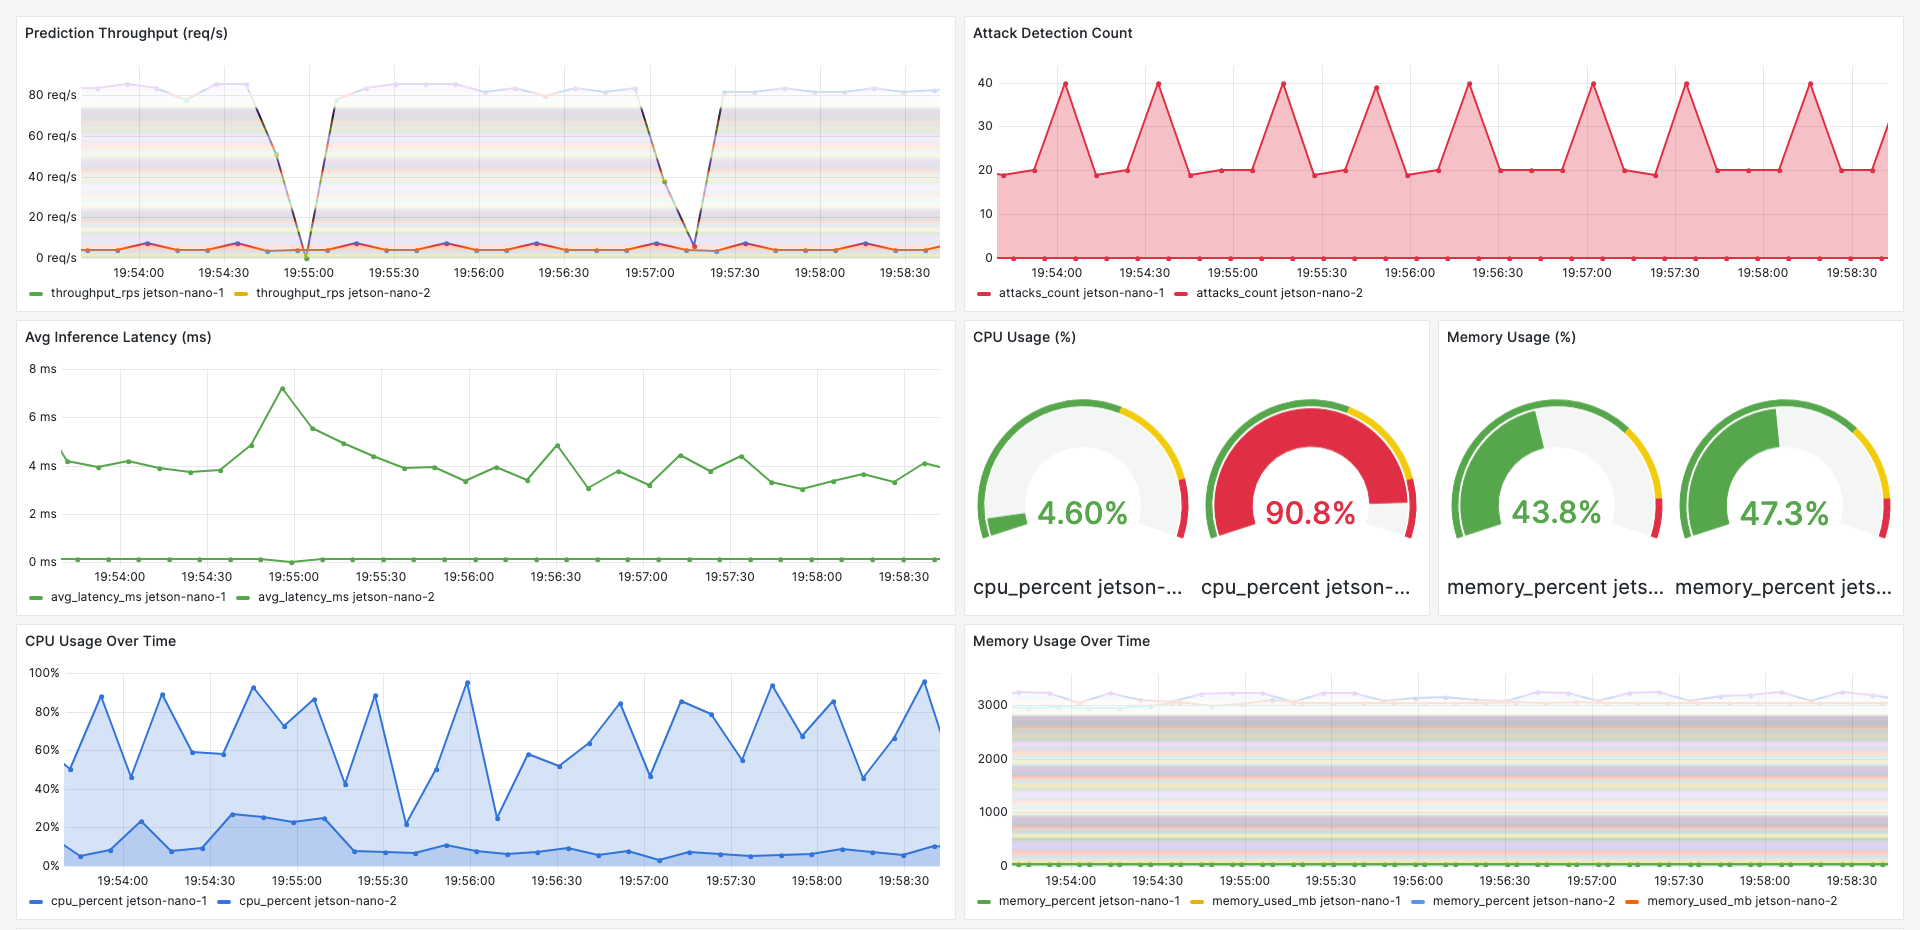
\includegraphics[width=\textwidth]{grafana_peak_load.png}
    \end{column}
    \begin{column}{0.35\textwidth}
      At peak load, split mode\\{\scriptsize (earlier run, previous model)}:
      \begin{itemize}
        \item gate node: \good{4.6\% CPU}
        \item classifier node: \bad{90.8\% CPU}
      \end{itemize}
      \vspace{0.5em}
      The classifier dominates the compute budget --- which is exactly why
      moving it off the ingest path pays.
    \end{column}
  \end{columns}
  \note{Live Grafana at peak load. Under five versus ninety-one percent. The
  asymmetry is the whole argument for the split. Add: the gate is a tunable
  filter, not a fixed point --- backup slide has the operating curve.}
\end{frame}

% ---------------------------------------------------------------- 0:35
\begin{frame}{Result 3: what the gate lets through}
  \begin{columns}[T]
    \begin{column}{0.52\textwidth}
      \centering\small
      \fitwidth{%
      \begin{tabular}{lccc}
        \toprule
        Gate threshold & Attacks & False & Flows \\
        (benign quantile) & forwarded & alarms & skipped \\
        \midrule
        0.99              & 72.4\% & 0.99\% & 88.3\% \\
        \textbf{0.995 (deployed)} & \num{68.1\%} & \num{0.49\%} & 89.4\% \\
        0.999             & 39.8\% & 0.09\% & 94.0\% \\
        \bottomrule
      \end{tabular}
      }
      \\[0.3em]
      \raggedright\scriptsize Offline, CICIDS2017 test split; gate on all 77
      features. Streamed live: 69.6\% of 1{,}261 attack flows caught.
    \end{column}
    \begin{column}{0.45\textwidth}
      \begin{itemize}\small
        \setlength{\itemsep}{0.4em}
        \item A flow the gate skips is final: \bad{about 30\% of attack flows}
              never reach the classifier.
        \item On the classifier's 30 features the gate would forward only
              44.8\%.
        \item The operator picks the point that fits the budget.
      \end{itemize}
    \end{column}
  \end{columns}
  \takeaway{The capacity gain is paid for in recall: the gate is a
  \key{tunable trade-off}, not a free filter.}
  \note{Numbers from results/ml\_08\_anomaly\_gate/gate\_operating\_points.csv;
  the deployed threshold is quantile 0.995. Without the gate, every attack flow
  in the replay was caught, so the loss is the gate's.}
\end{frame}

% ---------------------------------------------------------------- 0:45
\begin{frame}{Result 4: the price of one unified stack}
  We serve with Spark for \emph{consistency with distributed training}.
  What does that cost? The \emph{deployed forest}, exported, same board:
  \vspace{0.5em}
  \centering
  \small
  \fitwidth{%
  \begin{tabular}{lccc}
    \toprule
    Engine & Flows/s & Batch p95 (ms) & mJ per flow \\
    \midrule
    PySpark (deployed) & 1.4      & 7515  & 1506 \\
    NumPy              & 54.8     & 194   & 11.3 \\
    \textbf{ONNX Runtime} & \num{10{,}092} & \num{1.2} & \num{0.087} \\
    \bottomrule
  \end{tabular}
  }
  \\[0.2em]{\scriptsize Identical predictions on every flow. mJ per flow: energy
  above the board's idle power.}
  \takeaway{ONNX Runtime serves the same forest \num{$\approx$7{,}200$\times$}
  faster. Target for the next iteration: \key{train on Spark, serve with
  ONNX/TensorRT}.}
  \note{The JVM costs us more than three orders of magnitude, and that sets
  the roadmap. Batch size 10.}
\end{frame}

% ---------------------------------------------------------------- 0:40
\begin{frame}{Conclusion}
  \begin{columns}[T]
    \begin{column}{0.53\textwidth}
      \textbf{What we showed}
      \begin{itemize}
        \item A reproducible distributed edge IDS: Kafka $+$ PySpark on a
              Jetson Orin Nano Super cluster.
        \item Gate and classifier on separate boards:
              \good{2.5 $\rightarrow$ 22.4 flows/s} sustained, e2e p95
              $\approx$7\,s.
        \item Energy per verdict: \good{3.0\,J $\rightarrow$ 0.60\,J}.
        \item ONNX serves the same forest $\approx$7{,}200$\times$ faster.
      \end{itemize}
    \end{column}
    \begin{column}{0.44\textwidth}
      \textbf{Limitations}
      \begin{itemize}\footnotesize
        \item Two-node lab cluster over Wi-Fi; replayed traffic.
        \item Gate skips $\approx$30\% of attack flows.
        \item GPU unused (CPU-only pipeline); evasion untested.
      \end{itemize}
      \textbf{Next}
      \begin{itemize}\footnotesize
        \item ONNX/TensorRT serving; live traffic; retraining under drift.
      \end{itemize}
    \end{column}
  \end{columns}
  \vfill
  \centering
  \key{Thank you --- questions?}
  \note{Recap: nine times the load, five times less energy per verdict, and
  the price, about thirty percent of attacks skipped by the gate.}
\end{frame}

% ---------------------------------------------------------------- 7:00
\begin{frame}{Key references}
  \begin{itemize}\footnotesize
    \setlength{\itemsep}{0em}
    \item[{[1]}] Sharafaldin, I., Lashkari, A.\,H. \& Ghorbani, A.\,A.
          \emph{Toward generating a new intrusion detection dataset and
          intrusion traffic characterization}. ICISSP 2018.
          \hfill{\key{CICIDS2017}}
    \item[{[2]}] Shi, W. et al. \emph{Edge computing: Vision and challenges}.
          IEEE Internet of Things Journal 3(5), 2016.
          \hfill{\key{edge setting}}
    \item[{[3]}] Chandola, V., Banerjee, A. \& Kumar, V. \emph{Anomaly detection:
          A survey}. ACM Computing Surveys 41(3), 2009.
          \hfill{\key{anomaly gate}}
    \item[{[4]}] Lundberg, S.\,M. \& Lee, S.-I. \emph{A unified approach to
          interpreting model predictions}. NeurIPS 2017.
          \hfill{\key{SHAP Top-30}}
    \item[{[5]}] Zaharia, M. et al. \emph{Spark: Cluster computing with working
          sets}. HotCloud 2010.
          \hfill{\key{Spark}}
    \item[{[6]}] Kreps, J., Narkhede, N. \& Rao, J. \emph{Kafka: a Distributed
          Messaging System for Log Processing}. NetDB 2011.
          \hfill{\key{Kafka}}
    \item[{[7]}] Mohan Kiran Kumar, K. et al. \emph{Distributed Intrusion Detection
          System using Kafka and Spark Streaming}. ICVADV 2025.
          \hfill{\key{closest system}}
    \item[{[8]}] Arp, D. et al. \emph{Dos and Don'ts of Machine Learning in Computer
          Security}. USENIX Security 2022.
          \hfill{\key{leakage-aware protocol}}
  \end{itemize}
  \note{Not presented --- shown while taking questions, so sources are on
  screen if the audience asks. Full list is in the paper.}
\end{frame}

% =====================================================================
\appendix

\begin{frame}[standout]
  Backup slides
\end{frame}

\begin{frame}{Backup: sustained capacity and energy per mode}
  \centering
  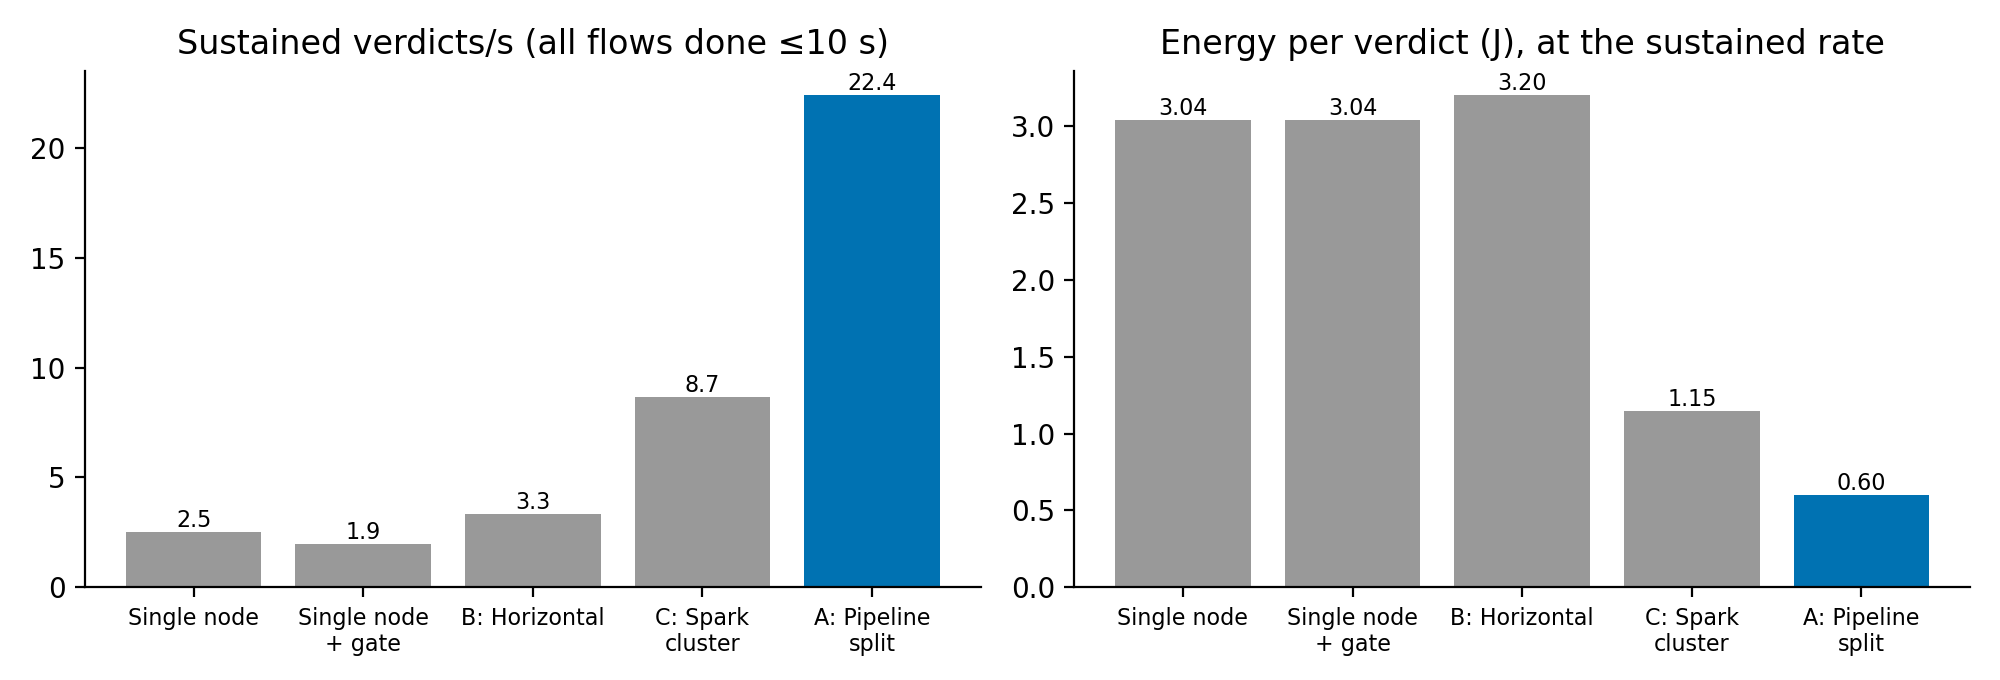
\includegraphics[height=0.70\textheight, width=\textwidth, keepaspectratio]{edge_capacity.png}
  \\[0.2em]
  \footnotesize Sustained verdicts/s with every flow done within 10\,s (left);
  energy per verdict at that rate (right).
\end{frame}

\begin{frame}{Backup: the gate is an operating curve, not a point}
  \centering
  \IfFileExists{../../results/ml_08_anomaly_gate/gate_operating_points.png}
    {\includegraphics[height=0.68\textheight, width=\textwidth, keepaspectratio]{gate_operating_points.png}}
    {\fbox{\parbox{0.7\textwidth}{\centering\vspace{1.5cm}
      \texttt{gate\_operating\_points.png}\vspace{1.5cm}}}}
  \\[0.2em]
  \footnotesize Attack recall (left) and false-positive rate (right) vs.\
  gate-skip ratio. Raising the skip ratio offloads more Spark work and costs
  recall; the operator chooses the point.
\end{frame}

\begin{frame}{Backup: which model, and why}
  \centering\small
  \fitwidth{%
  \begin{tabular}{lcccp{3.3cm}}
    \toprule
    Configuration & F1 & Features & Size (MB) & Edge rationale \\
    \midrule
    Baseline $+$ XGBoost      & 0.9971 & 77 & 2.32 & Reference accuracy \\
    \textbf{SHAP Top-30} $+$ XGBoost & 0.9970 & 30 & 0.003$^{\dagger}$ & Explainable; deployed feature set \\
    RF Top-30 $+$ XGBoost     & 0.9922 & 30 & 2.52 & Embedded ranking \\
    PCA $k$=40 $+$ XGBoost    & 0.9939 & 40 & 3.82 & Unsupervised reduction \\
    \bottomrule
  \end{tabular}
  }
  \\[0.4em]
  \raggedright\footnotesize
  We deploy \key{SHAP Top-30 with Random Forest} (exported model: test F1
  0.9959, 30 features): a native Spark ML estimator, so the
  \texttt{PipelineModel} loads on ARM64 without the native libraries Spark's
  XGBoost integration needs. The SHAP ranking is computed after
  \texttt{destination\_port} is removed.
  \\ $^{\dagger}$Distributed saving under-reports size; true size $\approx$2.5\,MB.
\end{frame}

\begin{frame}{Backup: full monitoring dashboard}
  \centering
  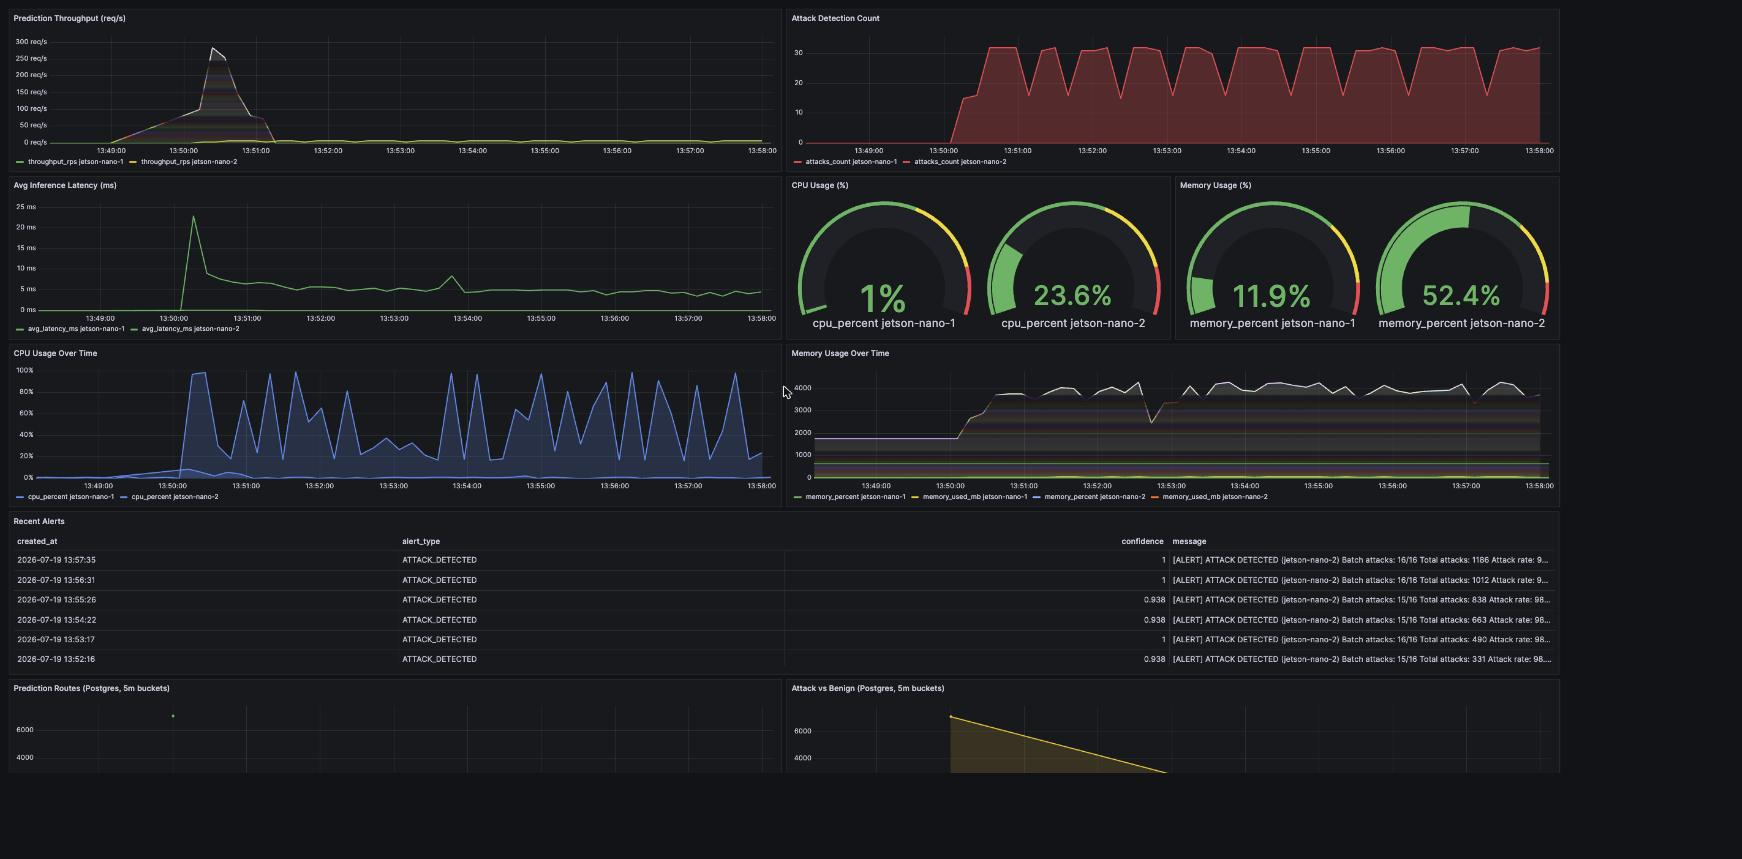
\includegraphics[height=0.70\textheight, width=\textwidth, keepaspectratio]{grafana_dashboard.png}
  \\[0.2em]
  \footnotesize Per-node throughput, detected attacks, inference latency,
  CPU/RAM for both boards, PostgreSQL-backed alerts.
\end{frame}

\begin{frame}{Backup: measurement protocol}
  \begin{itemize}\small
    \item Host-side orchestration starts pipeline roles on the Jetsons over
          SSH, drives the load, collects every verdict.
    \item Each verdict stores the flow's send time and replay row: latency is
          send to verdict, \emph{queueing included}; skip ratio and attack
          recall come from the flows themselves.
    \item Rate sweep per mode; a rate is sustained when every flow sent in the
          45\,s window gets its verdict within 10\,s after it. 2 runs per rate.
    \item Fresh Kafka consumer group per run, so no run inherits a backlog.
    \item Tiers batch 20 flows or flush after 1\,s.
    \item Energy: \texttt{tegrastats}, 30\,s idle baseline then load at the
          sustained rate; two-node modes sum both boards.
  \end{itemize}
\end{frame}

\end{document}
